% One-dimensional data
\subsection{One Dimension}
\subsubsection{Simple Reward Function}
As a very basic proof of concept, we ran the algorithms on the reward
function $r(x) = x$ over the unit interval [0,1].

\begin{figure}[!ht]
  \begin{center}
    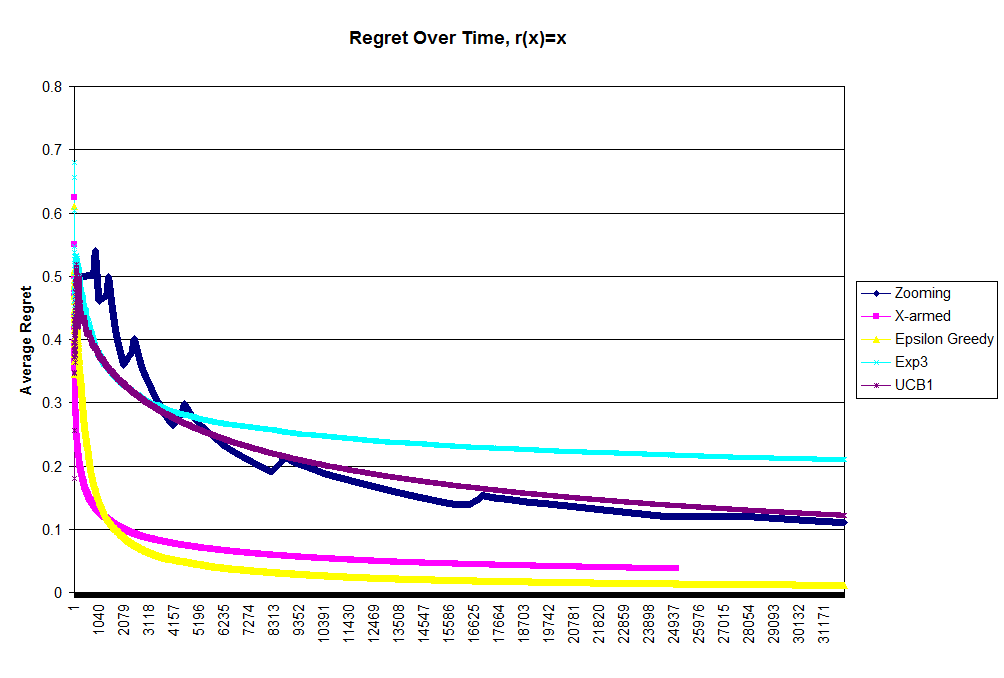
\includegraphics[width=\figwidth]{figures/1dsimpleplot.png}
     \caption{$r(x) = x$, 100 arms for discretization
     algorithms}
     \label{fig:1dsimple}
  \end{center}
\end{figure}

From figure \ref{fig:1dsimple}, we can see a number of facts.  First, at 
least in this case, the $\epsilon$-greedy algorithm is clearly the
best of all discretization algorithms, which is due to there being
no noise.  The $\mathcal{X}$-armed algorithm also does rather well,
but becomes expensive computationally as the number of rounds becomes
large due to having $O(n)$ time complexity in each round, where $t$ is
the number of rounds so far.  We can also see the characteristic bumps of
the Zooming algorithm, which are indicative of the fact that the Zooming
algorithm does not carry over information between phases.


\subsubsection{Noisy Reward Function}
Now we shall add some noise to our reward function.  The new reward
function is $r(x) = b(n_{0,1}(x))$, where $b(x) = 1$ with probability
$x$ and is 0 otherwise and $n_{\alpha_,\beta}(x)$ is $x$ times a random
number uniformly drawn from the interval $[\alpha, \beta]$.  The results
are presented in figure \ref{fig:1dnoise}

\begin{figure}[!ht]
  \begin{center}
    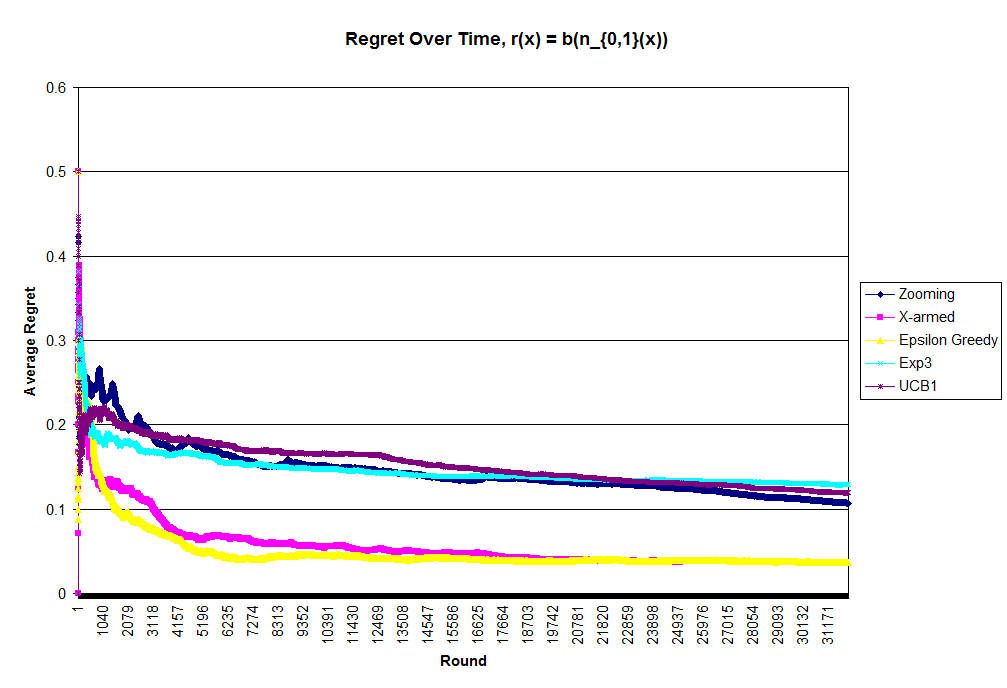
\includegraphics[width=\figwidth]{figures/1dnoiseplot.png}
     \caption{$r(x) = b(n_{0,1}(x))$, 100 arms for discretization
     algorithms}
     \label{fig:1dnoise}
  \end{center}
\end{figure}

For the most part, the algorithms perform basically as well as they did
in the no-noise case, with the notable exceptions that Exp3 algorithm did
better than before and the $\epsilon$-greedy algorithm did slightly worse
than before.  In the case of the $\epsilon$-greedy algorithm, this can be
partially attributed to the fact that the random discretization determines
how low the average regret can get, and that in this particular trial
the discretization was not very good.  We can tell that this is the true
reason for this behavior because otherwise, the $\epsilon$-greedy algorithm
would be converging more slowly, which does not appear to be the case.

Overall, from these simple 1D cases, we can see that
$\mathcal{X}$-armed algorithm appears to perform better than the Zooming
algorithm, although at the cost of being rather slow when the number of
rounds becomes large.  In a bandit setting, though, it is generally the
case that the reward function is somewhat costly to evaluate, and so the
computational cost of the $\mathcal{X}$-armed algorithm is not quite so
important.  Also, if we look at the very first few trials, the
$\mathcal{X}$-armed algorithm does fairly well rather quickly, whereas
the other algorithms take a little bit longer to fully explore the space.
For the discretization algorithms, though, this can be mitigated by
choosing a smaller number of arms to discretize the domain into.  In fact,
the very number of arms chosen for those algorithms is essentially a 
parameter helping to determine how much exploration to do -- more arms
will cause more exploration, and fewer arms will cause more exploitation.

\subsubsection{Prisoner's Dilemma - Changing Reward Function}
Here we present how the algorithms did against each other in an extension of
the Prisoner's Dilemma to a continuous-choice case.  As we shall have the
algorithms playing against each other, the reward function for a single
algorithm is not constant with respect to time, and so there is no reason to
suspect that the algorithms will still perform well, but it is an interesting
problem, even just to see the results.

First, we define our reward functions.  Given players 1 and 2, we define the
reward functions $r_1(x_1, x_2)$ and $r_2(x_1, x_2)$ by
\[
	r_1(x_1, x_2) = \frac{1}{3} x_1 - \frac{2}{3} x_2 + \frac{2}{3}
	r_2(x_1, x_2) = -\frac{2}{3} x_1 + \frac{1}{3} x_2 + \frac{2}{3}
\]
Note that each reward function is a plane, and that we have
\begin{gather*}
	(r_1(0,0), r_2(0,0)) = \left(\frac{2}{3}, \frac{2}{3}\right) \\
	(r_1(1,0), r_2(1,0)) = (1, 1) \\
	(r_1(0,1), r_2(0,1)) = (0, 1) \\
	(r_1(1,1), r_2(1,1)) = \left(\frac{1}{3}, \frac{1}{3}\right)
\end{gather*}
which is precisely the setup in a Prisoner's Dilemma game where 0 corresponds
to colluding and 1 corresponds to not colluding.

We use 100 arms for the discretization algorithms here, and each trial is run
through 5000 rounds.  We also introduce a modified $\mathcal{X}$-armed
algorithm which does a random walk down its covering tree with probability .1,
in the hopes that this will allow it to adapt to a changing reward function.
Here we present the average rewards over those rounds, where the first element
in a pair of numbers corresponds to the average reward for the row algorithm
and the second number corresponds to the average reward for the column
algorithm.  

\begin{tabular}{|c|c|c|c|c|c|c|}
\hline
& $\epsilon$-greedy & UCB1 & Exp3 & $\mathcal{X}$-armed &
Modified $\mathcal{X}$-armed & Zooming \\ \hline
$\epsilon$-greedy & .44, .39 & .60, .25 & .55, .27 & .47, .31 & .49, .35 &
.58, .25\\ \hline
UCB1 & & .48, .46 & .48, .46 & .37, .52 & .37, .49  & .46, .48 \\ \hline
Exp3 & & & .47, .44 & .36, .52 & .39, .46 & .48, .44 \\ \hline
$\mathcal{X}$-armed & & & & .59, .59 & .48, .49 & .53, .34 \\ \hline
Modified $\mathcal{X}$-armed & & & & & .50, .50 & .52, .35 \\ \hline
Zooming & & & & & & .53, .53 \\ \hline
\end{tabular}

As a sidenote, the algorithms that tended to do too much exploring in the
simple case of $r(x)=x$ tended to have the least convergence to an arm.
On the other hand, the $\epsilon$-greedy algorithm was relatively
convergent, almost always to relatively high values, which corresponds to
not colluding in the game and is the dominant strategy.  Also, the
deterministic algorithms, when run against themselves, obviously performed
identically to one another.  In particular, this causes the
$\mathcal{X}$-armed algorithm to always think that colluding is better, and
hence that matchup has the highest average rewards.
Now we shall examine the numbers.

Roughly speaking, the algorithms performed just about in the same order of
their performance on the simple $r(x)=x$ case.  This is somewhat surprising,
given that this reward function is not only slightly more complicated, but
changing over time.  In particular, the $\epsilon$-greedy algorithm was
just about always the best algorithm, the $\mathcal{X}$-armed algorithms
performed about the same, despite the modification, and the UCB1, Exp3,
and Zooming algorithms were all about the same.  Looking at the 5000
round mark in Figure \ref{fig:1dsimple}, this is an exact correlation, and
thus provides evidence for the hypothesis that the simple test cases
considered probably generalize in roughly a similar fashion, given how
different the reward function in this case was.
